\documentclass[a4paper]{article}
\usepackage[utf8]{inputenc}
\usepackage[spanish, es-tabla, es-noshorthands]{babel}
\usepackage[table,xcdraw]{xcolor}
\usepackage[a4paper, footnotesep = 1cm, width=22cm, top=2.5cm, height=25cm, textwidth=20cm, textheight=25cm]{geometry}
%\geometry{showframe}

\usepackage{tikz}
\usepackage{amsmath}
\usepackage{amsfonts}
\usepackage{amssymb}
\usepackage{float}
\usepackage{graphicx}
\usepackage{caption}
\usepackage{subcaption}
\usepackage{multicol}
\usepackage{multirow}
\usepackage{wrapfig}
\setlength{\doublerulesep}{\arrayrulewidth}
\usepackage{booktabs}

\usepackage{hyperref}
\hypersetup{
    colorlinks=true,
    linkcolor=blue,
    filecolor=magenta,      
    urlcolor=blue,
    citecolor=blue,    
}

\newcommand{\note}[1]{
	\begin{center}
		\huge{ \textcolor{red}{#1} }
	\end{center}
}

\setcounter{topnumber}{2}
\setcounter{bottomnumber}{2}
\setcounter{totalnumber}{4}
\renewcommand{\topfraction}{0.85}
\renewcommand{\bottomfraction}{0.85}
\renewcommand{\textfraction}{0.15}
\renewcommand{\floatpagefraction}{0.8}
\renewcommand{\textfraction}{0.1}
\setlength{\floatsep}{5pt plus 2pt minus 2pt}
\setlength{\textfloatsep}{5pt plus 2pt minus 2pt}
\setlength{\intextsep}{5pt plus 2pt minus 2pt}

\newcommand{\quotes}[1]{``#1''}
\usepackage{array}
\newcolumntype{C}[1]{>{\centering\let\newline\\\arraybackslash\hspace{0pt}}m{#1}}
\usepackage[american]{circuitikz}
\usetikzlibrary{calc}
\usepackage{fancyhdr}
\usepackage{units} 

\graphicspath{{../Ejercicio-1/}{../Ejercicio-2/}{../Ejercicio-3/}{../Ejercicio-4/}{../ParteI/}{../ParteII/}{../ParteIII/}{../ParteIV/}}

\pagestyle{fancy}
\fancyhf{}
\lhead{22.14 - Electrónica IV}
\rhead{Mechoulam, Lambertucci, Londero}
\rfoot{Página \thepage}


\begin{document}

\subsection{Introducción}

Se analizó la conmutación de un MOSFET \href{https://www.vishay.com/docs/91019/91019.pdf}{IRF530} de potencia en un circuito con carga inductiva, utilizando un diodo \href{https://www.onsemi.com/pdf/datasheet/mur420-d.pdf}{MUR460} de potencia para proporcionar un camino a la corriente durante el apagado del MOSFET y no dañar al circuito.

%Aca puede ir la foto del circuito

Para la conmutación del MOSFET se utilizó un periodo de $T_s = 20 \mu s$ y un duty cycle de $D = 50 \%$.

\subsection{Circuito en la Teoría}

En la teoría, se consideró al diodo MUR460 como ideal excepto por la caída de potencial de la juntura en directa, siendo esta extraída de la datasheet, con un valor de $V_{D_{on}} = 1.3V$. Además, se consideró a la bobina como ideal con resistencia serie nula.

\begin{figure}[H]
	\centering
	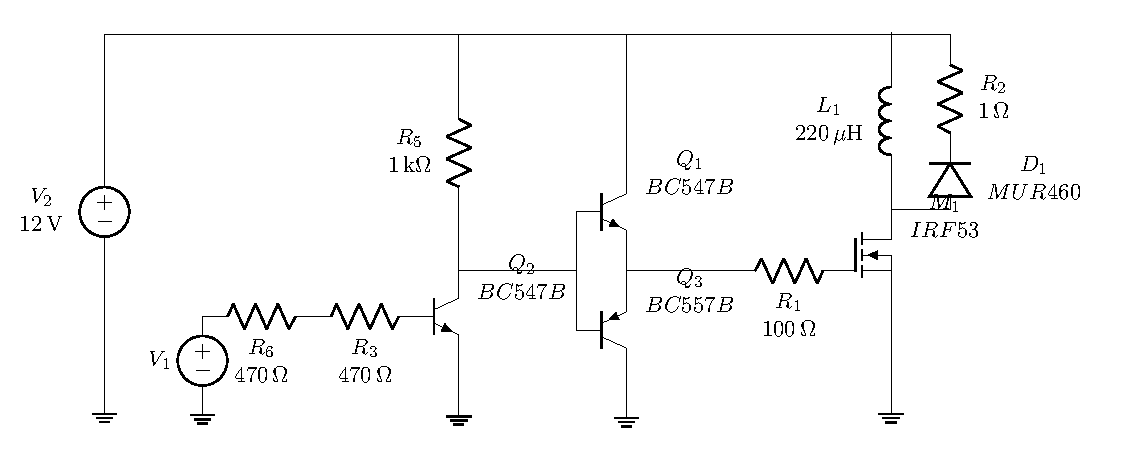
\includegraphics[width=0.7\linewidth, page=1]{ImagenesEjercicio-1/CircuitsEj1}
	\caption{Circuito para el estudio de la conmutación del MOSFET.}
	\label{ej1:fig:circuito}
\end{figure}

\subsubsection{Primer Hemicircuito: MOSFET ON}

Cuando el MOSFET se encuentra encendido, se forma un circuito RL entre la bobina y la $R_{ds_{on}}$ del MOSFET. Como el diodo se encuentra con su ánodo conectado a aproximadamente tierra, y su cátodo conectado a $V_i$, este se encuentra en inversa por lo que no circula corriente a través de él.

\begin{figure}[H]
	\centering
	\includegraphics[width=0.4\linewidth, page=3]{ImagenesEjercicio-1/CircuitsEj1}
	\caption{Hemicircuito con MOSFET encendido.}
	\label{ej1:fig:circuito_on}
\end{figure}

Resolviendo el circuito RL, se puede observar en las ecuaciones (\ref{ej1:eq:IL_on}) y (\ref{ej1:eq:VL_on}) que durante el MOSFET se encuentra encendido aumenta la energía almacenada en la bobina. Sobre el MOSFET caen $V_{ds_{on}} = I_{L_{on}}\cdot R_{ds_{on}}$

\begin{equation}
	 I_{L_{on}}(t) = \left( I_{L_{off}}\left(t= \frac{n}{f_{sw}}\right) -\frac{V_2}{R_{ds_{on}}+R_2}\right) e^{-\frac{R_{ds_{on}}+R_2}{L}t} + \frac{V_2}{R_{ds_{on}}+R_2} \ \ \ \ n \in \mathbb{N}
\label{ej1:eq:IL_on}
\end{equation}

\begin{equation}
	V_{L_{on}}(t) = \left( V_2 - I_{L_{off}}\left(t= \frac{n}{f_{sw}}\right)\cdot (R_{ds_{on}}+R_2) \right)e^{-\frac{R_{ds_{on}}+R_2}{L}t} \ \ \ \ n \in \mathbb{N}
\label{ej1:eq:VL_on}
\end{equation}

Donde $t=\frac{n}{f_{sw}}$ son los momentos en los que el MOSFET conmuta de apagado a encendido y $I_{L_{off}}\left(t= \frac{n}{f_{sw}}\right)$ la corriente en la bobina en dicho momento.

\subsubsection{Segundo Hemicircuito: MOSFET OFF}

Una vez apagado el MOSFET, la bobina posee la tensión $V_{L_{off}}$ necesaria entre sus bornes para que siga circulando la corriente $I_{L_on}$. Sobre el MOSFET caen $V_{ds_{off}} = V_2 + V_D = 13.3V$ circulando la malla formada por el diodo, el MOSFET y la fuente de entrada. En este estado, si se desprecia la corriente parásita del MOSFET, toda la corriente $I_{L_{off}}$ de la bobina pasa por el diodo el cual se encuentra polarizado en directa a consecuencia de la tensión impuesta por la bobina y no se extrae corriente de la fuente de alimentación.

\begin{figure}[H]
	\centering
	\includegraphics[width=0.4\linewidth, page=2]{ImagenesEjercicio-1/CircuitsEj1}
	\caption{Hemicircuito con MOSFET apagado.}
	\label{ej1:fig:circuito_off}
\end{figure}

Resolviendo el circuito RL que se obtiene en este estado, se observa que la bobina tiene una pérdida de energía almacenada dada por las ecuaciones (\ref{ej1:eq:IL_off}) y (\ref{ej1:eq:VL_off}).

\begin{equation}
	 I_{L_{off}}(t) = \left( I_{L_{on}}\left(t= \frac{nD}{f_{sw}}\right) -\frac{V_d}{R_2}\right) e^{-\frac{R_2}{L}t} + \frac{V_d}{R_2} \ \ \ \ n \in \mathbb{N}_o
\label{ej1:eq:IL_off}
\end{equation}

\begin{equation}
	 V_{L_{off}}(t) = \left( V_d - I_{L_{on}}\left(t= \frac{nD}{f_{sw}}\right)\cdot R_2 \right)e^{-\frac{R_2}{L}t} \ \ \ \ n \in \mathbb{N}_o
\label{ej1:eq:VL_off}
\end{equation}

Donde $t=\frac{nD}{f_{sw}}$ son los momentos en los que el MOSFET conmuta de encendido a apagado y $I_{L_{on}}\left(t= \frac{nD}{f_{sw}}\right)$ la corriente en la bobina en dicho momentos. 

\subsubsection{Análisis en Estado Permanente}

En electrónica, se define el estado permanente de un circuito como la condición en la cual los efectos transitorios ya no son importantes. Para el circuito en cuestión, tiempo variante con dos estados específicos, se llega al estado permanente cuando las señales del circuito se tornan completamente periódicas según el periodo de conmutación. 

Analizando la constante de tiempo $\frac{L}{R} = 189.6\mu s$ de los hemicircuitos conformados por la carga inductiva, se observa que ésta es una orden de magnitud mayor que el tiempo que se transcurre en cada estado $t_{on} = t_{off} = \frac{D}{f_{sw}} = \frac{0.5}{60kHz} = 8.333\mu s$ por lo que se pueden aproximar la tensión $V_L$ como constante y la corriente $I_L$ como rectas de pendiente $\frac{V_L}{L}$. Para hallar la corriente media $\bar{I_L}$ de la bobina se realiza el promedio ponderado por el duty cycle de conmutado de los estados permanentes de ambos hemicircuitos, quedando

\begin{equation}
	\bar{I_L} = I_{L_{on}}(t \rightarrow \infty) \cdot D + I_{L_{off}}(t \rightarrow \infty) \cdot (1-D) = \frac{12V}{1\Omega + 0.16\Omega} \cdot 0.5 + 0V \cdot (1-0.5) = 5.17A
\end{equation}

Esto puede también resolverse de manera gráfica considerando las Ecuaciones (\ref{ej1:eq:IL_on}) y (\ref{ej1:eq:IL_off}) de las corrientes de la bobina para cada hemicircuito. En la Figura (\ref{ej1:fig:ILmediagrafico}) se observa que el cruce de ambas envolventes será la solución para la corriente media en la bobina en régimen permanente de conmutación.

\begin{figure}[H]
	\centering
	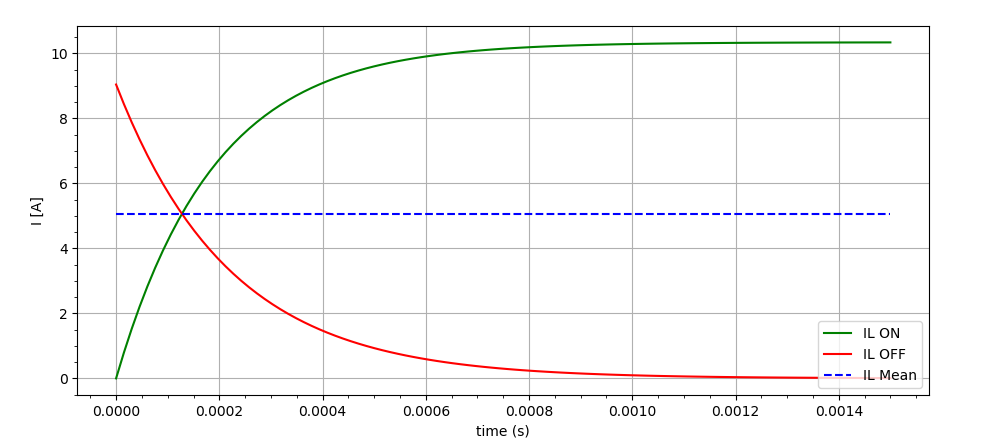
\includegraphics[width=0.5\linewidth]{ImagenesEjercicio-1/solgraficaIL}
	\caption{Solución gráfica de la corriente media en la bobina en régimen permanente.}
	\label{ej1:fig:ILmediagrafico}
\end{figure}

Conociendo la corriente media de la bobina, aproximando la tensión en cada estado como constante y teniendo en cuenta que la tensión media en los bornes de una inductancia debe ser nula en régimen permanente, se deduce que la forma de onda de $V_L$ será aproximadamente cuadrada, con una amplitud de $V_{max} = -V_{min} \approx V_D + \bar{I_L}R_2 = 6.47V$ observando la malla formada en la Figura (\ref{ej1:fig:circuito_off}). El ripple en la corriente $I_L$ será 

\begin{equation}
\Delta I_L = \frac{V_{max}}{L}\frac{D}{f_{sw}} = 245.1mA
\end{equation}

y el ripple en la tensión $V_L$ puede hallarse según la Ecuación (\ref{ej1:eq:VL_on}) como

\begin{equation}
\Delta V_L = \left( V_2 - \bar{I_L} (R_{ds_{on}}+R_2) \right) \cdot (1-e^{-\frac{R_{ds_{on}} + R_2}{L}\frac{D}{f_{sw}}}) = 258mV
\end{equation}

Finalmente, la corriente en el diodo $I_{diodo}$ será igual a la corriente en la bobina cuando el MOSFET se encuentra apagado, y nula cuando el MOSFET se encuentra prendido. La tensión $V_{ds}$ del MOSFET será igual a $13.3V$ durante el estado apagado como calculado en la sección anterior y $I_{L_{on}}(t)R_{ds_{on}} \approx \bar{I_L}R_{ds_{on}} = 827.2mV$ durante el estado encendido.

\subsubsection{Análisis de los Tiempos de Conmutación: Encendido}

Al encender el MOSFET con un escalón de tensión de $V_{GG} = 12V$, tomado en el borne izquierdo de $R_1$ y referido a masa, crece la corriente de gate $I_G$ instantáneamente a un valor de $I_G = \frac{V_i}{R_1} = 0.12A$ para luego decrecer exponencialmente según (\ref{ej1:eq:ig_ton}). Al mismo tiempo, la tensión entre gate y source pasa de ser nula a crecer exponencialmente según (\ref{ej1:eq:vgs_ton}).

\begin{equation}
I_G(t) = \frac{V_{GG}}{R_1}e^{-\frac{t}{\tau_1}}
\label{ej1:eq:ig_ton}
\end{equation}

\begin{equation}
V_{gs}(t) = V_{GG}(1-e^{-\frac{t}{\tau_1}})
\label{ej1:eq:vgs_ton}
\end{equation}

Donde la constante de tiempo $\tau_1 = R_1 (C_{gs}+C_{gd_{1}}) = 75ns$ es regida por la capacitancia de entrada del MOSFET compuesta por la capacitancia entre gate y source y la capacitancia entre gate y drain, con un valor de $C_{gs}+C_{gd_{1}} = 750pF$ observado en la Figura (\ref{ej1:fig:cgd}). Cuando la tensión entre gate y source llega al valor de threshold $V_{gs_{th}} = 4V$ (proporcionada por la datasheet del IRF530) luego de un tiempo 
\begin{equation}
t_{d_{on}} = -\tau_1 ln\left( 1-\frac{V_{th}}{V_2} \right) = 30.41ns
\label{ej1:eq:tdon}
\end{equation}

según la Ecuación (\ref{ej1:eq:vgs_ton}), comienza a crecer la corriente de drain $I_{ds}$ con pendiente constante. Una vez que la corriente de drain $I_{ds}$ alcanza el valor medio de la corriente de la bobina $\bar{I_L}$, se observa en la Figura (\ref{ej1:fig:vgsio}) proporcionada por la datasheet del IRF530 que la tensión $V_{gs}$ será $V_{gs_{io}} = 5.5V$. Utilizando este valor y la Ecuación (\ref{ej1:eq:vgs_ton}) se obtiene que el tiempo de rise de la corriente de drain es

\begin{equation}
	t_{ri} = -\tau_1 ln\left( 1-\frac{V_{gs_{io}}}{V_2} \right) -t_{d_{on}} = 15.57ns
\label{ej1:eq:trise}
\end{equation}

A partir de este momento, se formará la zona de depleción de la body layer por lo que la tensión $V_{ds}$ comenzará a caer. La tensión $V_{gs} = V_{gs_{io}}$ y la corriente $I_G = \frac{V_{GG}-V_{gs_{io}}}{R_1} = 65mA$ se mantendrá constante mientras la capacitancia $C_{gd}$ se incrementa de $C_{gd_1}$ a $C_{gd_2}$ debido a la formación de la susodicha zona de depleción. Luego de un tiempo $t_{fv}$ en el que fluyó una carga de $\Delta Q = 7.3nC$ al gate del MOSFET, dato proporcionado de la datasheet del IRF530 visto en la Figura (\ref{ej1:fig:deltaq}), la tensión $V_{ds}$ alcanzará un valor $V_{ds} = V_{ds_{on}} = \bar{I_L} R_{ds_{on}} = 827.59mV$ utilizando el valor de $\bar{I_L}$ calculado en la Ecuación (). El tiempo transcurrido en esta transición puede calcularse teniendo en cuenta la corriente $I_G = \frac{V_2 - V_{gs_{io}}}{R_1}$ obteniendo

\begin{equation}
	t_{fv} = \frac{R_1 \Delta Q}{V_2 - V_{gs_{io}}} = 112.31ns
	\label{ej1:eq:tfv}
\end{equation}

Finalmente, habiendo transicionado la capacitancia $C_{gd}$ de $C_{gd_1}$ a $C_{gd_2}$, se terminará de cargar la capacitancia de entrada del MOSFET según las Ecuaciones (\ref{ej1:eq:vgs_ton_2}) y (\ref{ej1:eq:ig_ton_2}).

\begin{equation}
V_{gs}(t) = V_{GG}(1-e^{-\frac{t}{\tau_2}})
\label{ej1:eq:vgs_ton_2}
\end{equation}

\begin{equation}
I_{G}(t) =  \frac{V_{GG}-V_{gs_{io}}}{R_1}e^{-\frac{t}{\tau_2}}
\label{ej1:eq:ig_ton_2}
\end{equation}

siendo $\tau_2 = R_1(C_{gs} + C_{gd_2})$ donde $C_{gs} + C_{gd_2} = 1150pF$ observado en la Figura (\ref{ej1:fig:cgd}). Se puede observar en las Figuras (\ref{ej1:fig:encendido_gate}) y (\ref{ej1:fig:encendido_drain}) el proceso entero de encendido descrito anteriormente.

\begin{figure}[H]
	\centering
	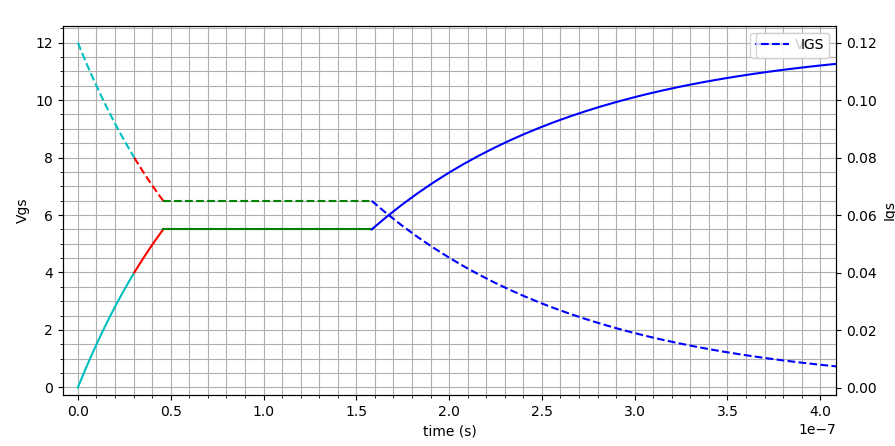
\includegraphics[width=0.8\linewidth]{ImagenesEjercicio-1/encendido_gate}
	\caption{$V_{gs}$ e $I_G$ en el encendido del MOSFET.}
	\label{ej1:fig:encendido_gate}
\end{figure}

\begin{figure}[H]
	\centering
	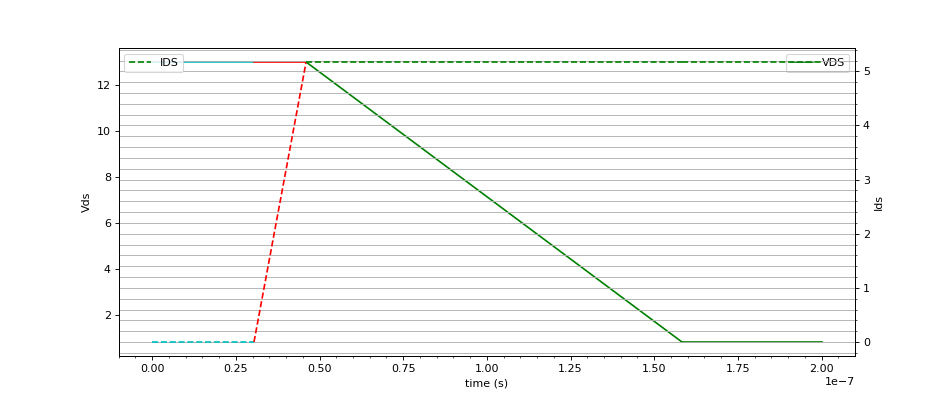
\includegraphics[width=0.8\linewidth]{ImagenesEjercicio-1/encendido_drain}
	\caption{$V_{ds}$ e $I_D$ en el encendido del MOSFET.}
	\label{ej1:fig:encendido_drain}
\end{figure}

\begin{figure}[H]
	\centering
	\begin{minipage}{0.45\textwidth}
		\centering
		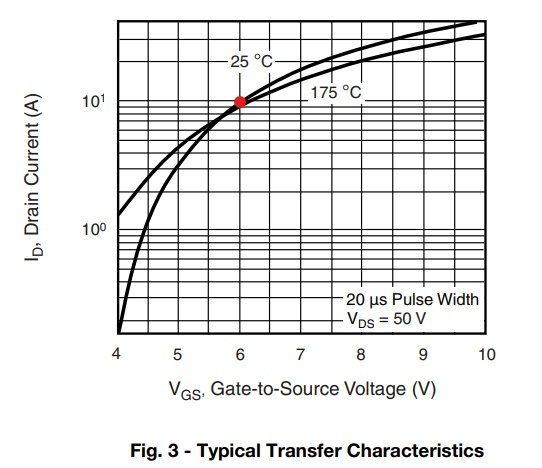
\includegraphics[width=\textwidth]{ImagenesEjercicio-1/Vgs-Id_LI} % first figure itself
		\caption{$V_{gs_{io}}$ de la datasheet del IRF530.}
		\label{ej1:fig:vgsio}
	\end{minipage}\hfill
	\begin{minipage}{0.45\textwidth}
		\centering
		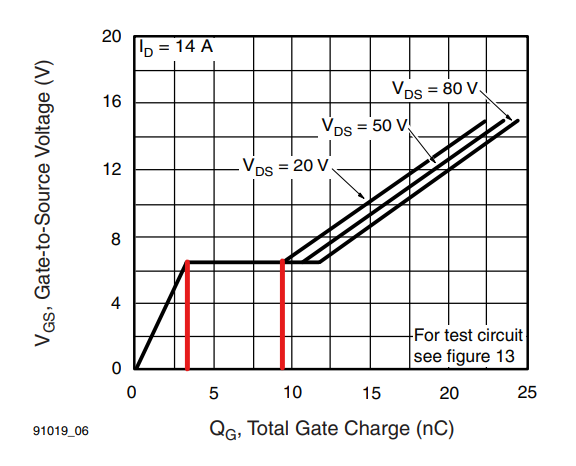
\includegraphics[width=\textwidth]{ImagenesEjercicio-1/deltaq} % second figure itself
		\caption{$\Delta Q$ en la transición de $C_{gd_1}$ a $C_{gs_2}$ de la datasheet del IRF530.}
		\label{ej1:fig:deltaq}
	\end{minipage}
\end{figure}

\begin{figure}[H]
	\centering
	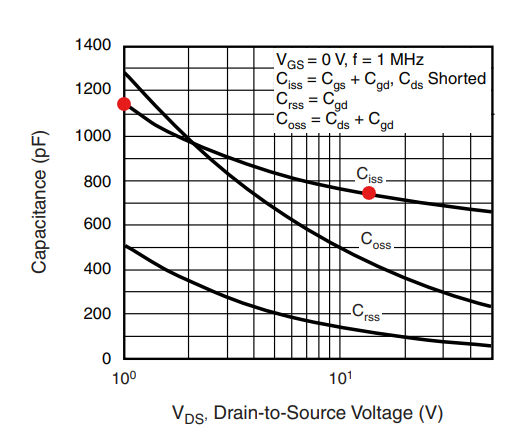
\includegraphics[width=0.4\linewidth]{ImagenesEjercicio-1/Vds-C}
	\caption{Capacitancia de entrada del MOSFET según la datasheet del IRF530 donde no ingresa carga a $C_{gs}$ debido a la tensión constante $V_{gs}$.}
	\label{ej1:fig:cgd}
\end{figure}

\subsubsection{Análisis de los Tiempos de Conmutación: Apagado}

\subsubsection{Corriente en el Diodo}

\subsubsection{Corriente en la Bobina}

\subsection{Circuito en la Simulación}

\subsection{Circuito en la Práctica}

\subsection{Diferencias}

\subsection{Conclusiones}

\end{document}